\documentclass[journal, a4paper]{IEEEtran}

% some very useful LaTeX packages include:

%\usepackage{cite}      % Written by Donald Arseneau
                        % V1.6 and later of IEEEtran pre-defines the format
                        % of the cite.sty package \cite{} output to follow
                        % that of IEEE. Loading the cite package will
                        % result in citation numbers being automatically
                        % sorted and properly "ranged". i.e.,
                        % [1], [9], [2], [7], [5], [6]
                        % (without using cite.sty)
                        % will become:
                        % [1], [2], [5]--[7], [9] (using cite.sty)
                        % cite.sty's \cite will automatically add leading
                        % space, if needed. Use cite.sty's noadjust option
                        % (cite.sty V3.8 and later) if you want to turn this
                        % off. cite.sty is already installed on most LaTeX
                        % systems. The latest version can be obtained at:
                        % http://www.ctan.org/tex-archive/macros/latex/contrib/supported/cite/

\usepackage{graphicx}   % Written by David Carlisle and Sebastian Rahtz
                        % Required if you want graphics, photos, etc.
                        % graphicx.sty is already installed on most LaTeX
                        % systems. The latest version and documentation can
                        % be obtained at:
                        % http://www.ctan.org/tex-archive/macros/latex/required/graphics/
                        % Another good source of documentation is "Using
                        % Imported Graphics in LaTeX2e" by Keith Reckdahl
                        % which can be found as esplatex.ps and epslatex.pdf
                        % at: http://www.ctan.org/tex-archive/info/

%\usepackage{psfrag}    % Written by Craig Barratt, Michael C. Grant,
                        % and David Carlisle
                        % This package allows you to substitute LaTeX
                        % commands for text in imported EPS graphic files.
                        % In this way, LaTeX symbols can be placed into
                        % graphics that have been generated by other
                        % applications. You must use latex->dvips->ps2pdf
                        % workflow (not direct pdf output from pdflatex) if
                        % you wish to use this capability because it works
                        % via some PostScript tricks. Alternatively, the
                        % graphics could be processed as separate files via
                        % psfrag and dvips, then converted to PDF for
                        % inclusion in the main file which uses pdflatex.
                        % Docs are in "The PSfrag System" by Michael C. Grant
                        % and David Carlisle. There is also some information
                        % about using psfrag in "Using Imported Graphics in
                        % LaTeX2e" by Keith Reckdahl which documents the
                        % graphicx package (see above). The psfrag package
                        % and documentation can be obtained at:
                        % http://www.ctan.org/tex-archive/macros/latex/contrib/supported/psfrag/

%\usepackage{subfigure} % Written by Steven Douglas Cochran
                        % This package makes it easy to put subfigures
                        % in your figures. i.e., "figure 1a and 1b"
                        % Docs are in "Using Imported Graphics in LaTeX2e"
                        % by Keith Reckdahl which also documents the graphicx
                        % package (see above). subfigure.sty is already
                        % installed on most LaTeX systems. The latest version
                        % and documentation can be obtained at:
                        % http://www.ctan.org/tex-archive/macros/latex/contrib/supported/subfigure/

\usepackage{url}        % Written by Donald Arseneau
                        % Provides better support for handling and breaking
                        % URLs. url.sty is already installed on most LaTeX
                        % systems. The latest version can be obtained at:
                        % http://www.ctan.org/tex-archive/macros/latex/contrib/other/misc/
                        % Read the url.sty source comments for usage information.

%\usepackage{stfloats}  % Written by Sigitas Tolusis
                        % Gives LaTeX2e the ability to do double column
                        % floats at the bottom of the page as well as the top.
                        % (e.g., "\begin{figure*}[!b]" is not normally
                        % possible in LaTeX2e). This is an invasive package
                        % which rewrites many portions of the LaTeX2e output
                        % routines. It may not work with other packages that
                        % modify the LaTeX2e output routine and/or with other
                        % versions of LaTeX. The latest version and
                        % documentation can be obtained at:
                        % http://www.ctan.org/tex-archive/macros/latex/contrib/supported/sttools/
                        % Documentation is contained in the stfloats.sty
                        % comments as well as in the presfull.pdf file.
                        % Do not use the stfloats baselinefloat ability as
                        % IEEE does not allow \baselineskip to stretch.
                        % Authors submitting work to the IEEE should note
                        % that IEEE rarely uses double column equations and
                        % that authors should try to avoid such use.
                        % Do not be tempted to use the cuted.sty or
                        % midfloat.sty package (by the same author) as IEEE
                        % does not format its papers in such ways.

\usepackage{amsmath}    % From the American Mathematical Society
                        % A popular package that provides many helpful commands
                        % for dealing with mathematics. Note that the AMSmath
                        % package sets \interdisplaylinepenalty to 10000 thus
                        % preventing page breaks from occurring within multiline
                        % equations. Use:
%\interdisplaylinepenalty=2500
                        % after loading amsmath to restore such page breaks
                        % as IEEEtran.cls normally does. amsmath.sty is already
                        % installed on most LaTeX systems. The latest version
                        % and documentation can be obtained at:
                        % http://www.ctan.org/tex-archive/macros/latex/required/amslatex/math/



% Other popular packages for formatting tables and equations include:

%\usepackage{array}
% Frank Mittelbach's and David Carlisle's array.sty which improves the
% LaTeX2e array and tabular environments to provide better appearances and
% additional user controls. array.sty is already installed on most systems.
% The latest version and documentation can be obtained at:
% http://www.ctan.org/tex-archive/macros/latex/required/tools/

% V1.6 of IEEEtran contains the IEEEeqnarray family of commands that can
% be used to generate multiline equations as well as matrices, tables, etc.

% Also of notable interest:
% Scott Pakin's eqparbox package for creating (automatically sized) equal
% width boxes. Available:
% http://www.ctan.org/tex-archive/macros/latex/contrib/supported/eqparbox/

% *** Do not adjust lengths that control margins, column widths, etc. ***
% *** Do not use packages that alter fonts (such as pslatex).         ***
% There should be no need to do such things with IEEEtran.cls V1.6 and later.


% Your document starts here!
\begin{document}

% Define document title and author
    \title{Midterm Report: Predictive Analysis of City Crime Hotspots}
    \author{Sahil Deshpande, Vinit Kumar \\ $\{sahilsd, vinitn\}@bu.edu$}
    \maketitle

% Write abstract here
\begin{abstract}
    With increased digitization of data around the world, various type of data is now easily available. This includes criminal reports for most of the major cities in the US. In order to constructively use this data and the available data mining tools in Python, we are trying to analyze crime hotspots and predict next most likely crime location. 
\end{abstract}

% Each section begins with a \section{title} command
\section{Introduction}
   Crimes have become a common part of city life that seriously affect quality of life and economic growth of a society. Universal organizations are spending a lot of resources trying to identify safest and most dangerous cities to help local authorities manage their workforce. As more and more people shift to the city, this concentrated population makes it important to find safer places. Using the open-source data from official websites and some of the basic data mining approaches, we are attempting to help this process [1].  

   From past analysis of various cities and their neighbourhoods, it has been shown that certain parts of the city are more prone to criminal activities than others making them a criminal hotspot. Even though there doesn't seem to be an intuitive pattern for criminals, they tend to favor certain areas that makes it possible to predict such malicious activities. Using the information about past activities, law enforcements can effectively serve their duties. 

   To achieve this predictive analysis, we have looked at various datasets available for free on the Internet[2-3]. After some research on which cities have most relevant and most updated data, we have decided to work with Boston, Los Angeles and Raleigh. The first part of this project is to get the data in a specified format (in this case json) and parse it to extract meaningful information. Using these parsed data structures, we are interested in finding the most relevant crime types such as assault, robbery, hit and run, to name a few. We select the types that affect a particular area the most using regression techniques[4]. After trimming the dataset, we have applied k-means clustering to plot these various types of activities using GMplot[5]. We now plan to use classification methods in order to predict most vulnerable parts of the city. Later sections describe the results we've seen so far.
% Main Part
    \begin{figure}[!hbt]
        % Center the figure.
        \begin{center}
        % Include the eps file, scale it such that it's width equals the column width. You can also put width=8cm for example...
        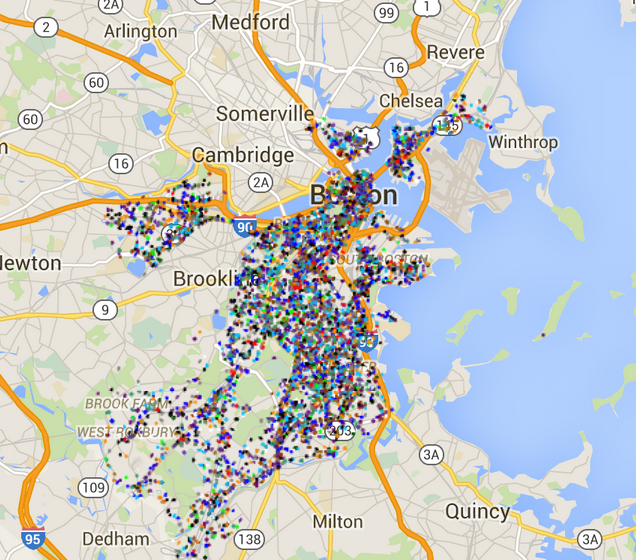
\includegraphics[width=\columnwidth]{fig1.png}
        % Create a subtitle for the figure.
        \caption{Overall crime distribution across Boston shows concentrated crime data.}
        % Define the label of the figure. It's good to use 'fig:title', so you know that the label belongs to a figure.
        \label{fig:tf_plot}
        \end{center}
    \end{figure}

    \begin{figure}[!hbt]
        % Center the figure.
        \begin{center}
        % Include the eps file, scale it such that it's width equals the column width. You can also put width=8cm for example...
        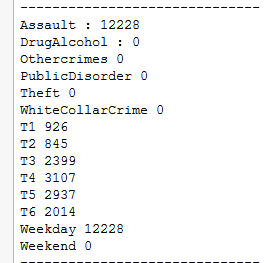
\includegraphics[width=\columnwidth]{fig2.png}
        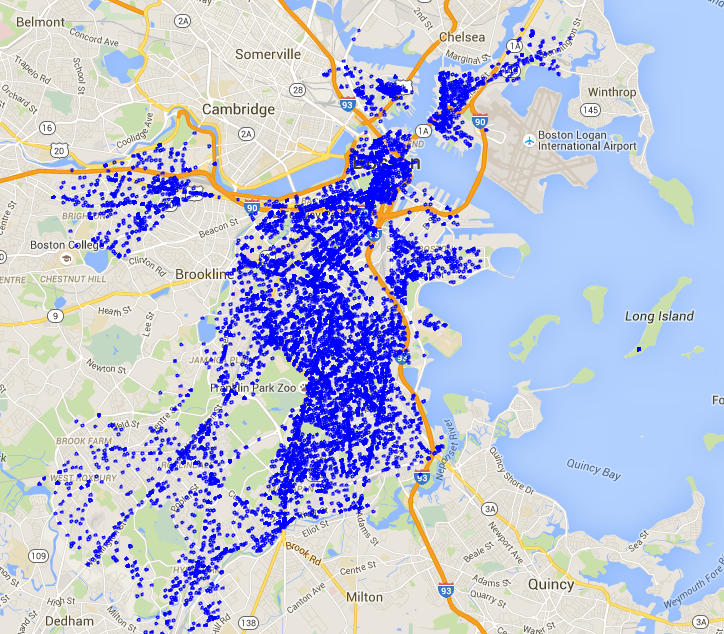
\includegraphics[width=\columnwidth]{fig3.png}
        % Create a subtitle for the figure.
        \caption{Cluster showing only Assault crimes and only on weekdays.}
        % Define the label of the figure. It's good to use 'fig:title', so you know that the label belongs to a figure.
        \label{fig:tf_plot}
        \end{center}
    \end{figure}

\section{Technique}

    \begin{figure}[!hbt]
        \begin{center}
        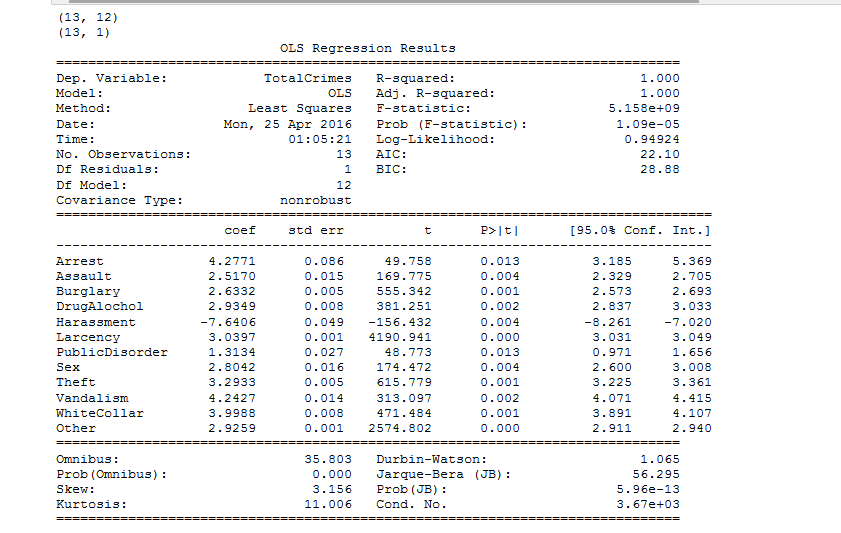
\includegraphics[width=\columnwidth]{regression.png}
        \caption{Linear Regression output for different types of crimes.}
        \label{fig:tf_plot}
        \end{center}
    \end{figure}

    First we searched on the Internet for reliable data sources for criminal activities in major cities in US. After going through large number of datafiles, we decided to work with data from [3]. After getting the data in json format, we parsed it to get attributes such as crime location, latitude and longitude, time of crime, day of the week, type of the crime. Since these attributes help us distinguish between most of the important crime activities, we plan to use these attributes for further analysis. 

    While parsing the data, we have also divided the timestamps into six categories and day of the week as weekday or weekend. This further enables more meaningful clustering because coarse datasets are clustered more effectively.

    In order to reduce this large data, have to used linear and logistic regression to find which crime types affect an area the most. Here we can calculate an average score for one area based on crime types (as we did in homework) and get top five coefficients that will denote the most common crime types. As we know, more data helps in better analysis and prediction we wanted to minimize this data reduction and thought this technique would be most effective.

    We first categorize the data in types like assault, robbery, disturbance, white collar crime and others. But this can be easily replaced with the types we get from regression results so we are first focusing on analysis part. Using these categories, we have applied K-means clustering from Python sklearn. The clustering results are explained in the next section. We have normalized the latitude and longitude during clustering so that they don't add any extra weight. While plotting the clusters on the map, we have used the original latitudes and longitudes to give correct crime hotspots.

    So this has given us a basic idea of malicious activities and their patterns in Boston. We can easily identify which areas show more assaults or weekend crime. This example already starts to unfold the advantages after seeing which areas are relatively safer and which would need more attention of local law enforcement. Using this clustered data, we are now exploring classifier methods in python which were discussed in the class. Right now we have come up with two approaches on how we can predict a crime but this part needs more work. First approach is to directly use latitude/longitude for predicting most likely crime activity but this has very fine granularity which makes it less favorable. On the other hand, we are planning to utilize area codes in the data set. This divide the city in certain code like A4, G1, etc. We can use these and one of the six timestamps and try to get a tuple similar to, $<$type of crime, area code, time category, day category$>$. We think this will be more clear after the Amazon prediction assignment. We plan to revisit this once more.
    



\section{Analysis of Crimes}
\subsection{Boston vs Los Angeles}
    \begin{figure}[!hbt]
        \begin{center}
        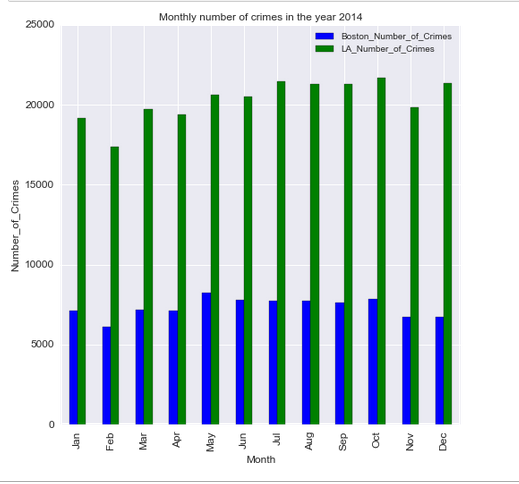
\includegraphics[width=\columnwidth]{boston-la-total.png}
        \caption{Total number of crimes in Boston and Los Angeles.}
        \label{fig:tf_plot}
        \end{center}
    \end{figure}
This graph clearly shows that Boston is a much safer city to live in as compared to LA and for every month, the number of crimes experienced for both the cities is pretty much constant. Even though this is not normalized with population, this seems to give some idea about crimes occurring in these two cities. In the month of February, the peak winter probably shows a slight dip in the number of crimes.

\subsection{Clustering}
    \begin{figure}[!hbt]
        \begin{center}
        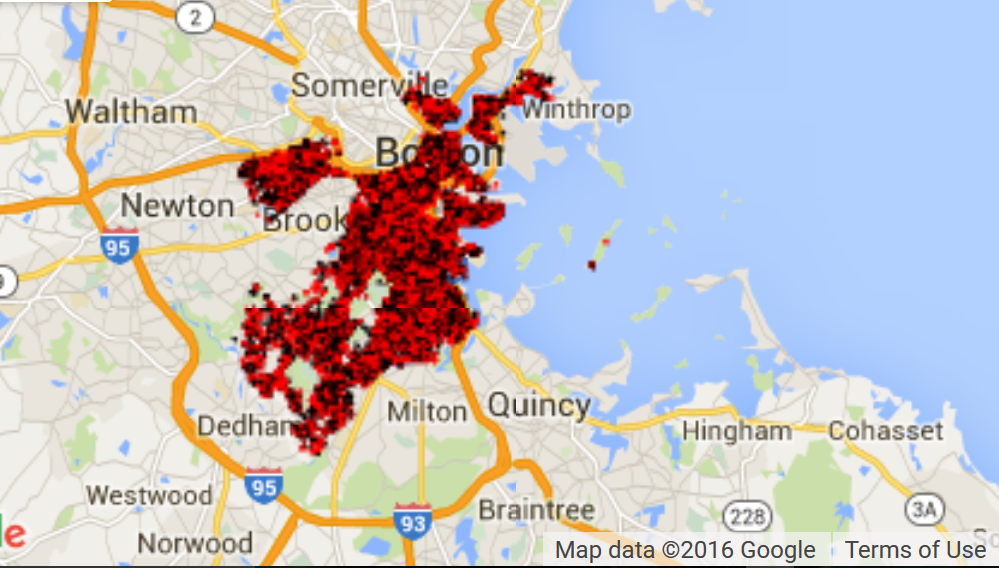
\includegraphics[width=\columnwidth]{boston-cluster-day.png}
        \caption{Clustering data based on weekday and weekend crimes.}
        \label{fig:tf_plot}
        \end{center}
    \end{figure}

The main idea of clustering was to determine the similar areas in the city bases on the type of crime that occurred, the time when it occurred and whether it occurred on a weekend or a weekday. We have removed few unnecessary crimes which occurred very few number of times and put few important crimes in the “Other” crime category. Though these crimes occurred few times, they are major crimes.
For clustering, we have used K-means++ algorithm. To determine the number of clusters, we computed the clustering and their associated error using k=1 through k=30. Using the output of the graph above, 15 is the number where error ceases to decrease by a significant amount. Hence, we have taken the number of clusters to be 15. 
We copied the dataframe with original values of latitude and longitude, normalized latitude and longitude into a new dataframe. We then actual latitude and longitude into the data frame and also the kmeans label. Based on the kmeans label, we created subsets of dataframes and used gmplot to plot the clusters on the google map.

\subsection{Clustering}
    \begin{figure}[!hbt]
        \begin{center}
        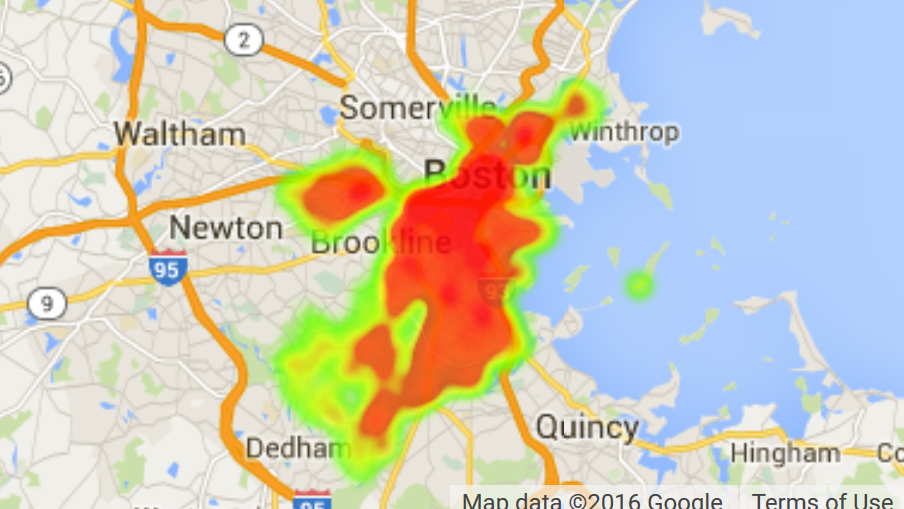
\includegraphics[width=\columnwidth]{boston-heatmap.png}
        \caption{Heatmap of Larceny and Assault crimes in Boston.}
        \label{fig:tf_plot}
        \end{center}
    \end{figure}

Above figure shows the crime areas, where crimes occurred during the mid-night time 9pm – 12 am.  The black spots indicate the areas where crimes occurred during weekend. The red spots indicate the areas where crimes occurred during weekday.



\subsection{Regression}
For Regression Analysis, we divided the data for each area code and got the total number of crime for each crime type, time of the day and type of the day. The aim of our regression analysis was to find to out what are the most important factors for the total number of crimes occurring in an area and what are the factors favorable for an area to be safe.

    \begin{figure}[!hbt]
        \begin{center}
        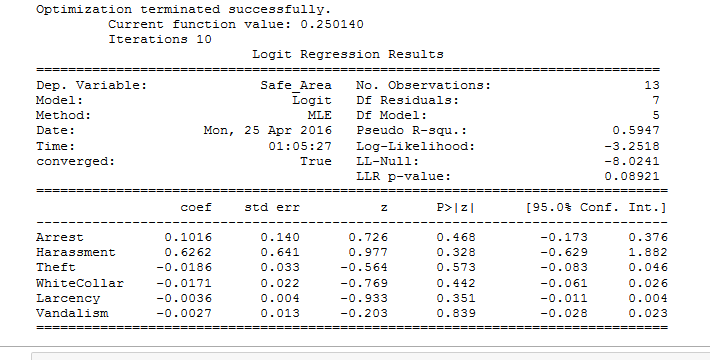
\includegraphics[width=\columnwidth]{logistic-reg-boston.png}
        \caption{Logistic Regression output for different types of crimes.}
        \label{fig:tf_plot}
        \end{center}
    \end{figure}

In Figure 3 we observe that the number of Harassment crimes has a negative correlation with the total number of crimes. This means the areas which have high number of Harassment crimes have a less total number of crimes.
From Figure 4, we can see that for the safe areas the only crime type that occurs in a significant number is Harassment.
Arrest and Vandalism have a high positive correlation as compared to other types. This implies the areas which have more Arrest and Vandalism crimes have more chances to be unsafe areas. 


\section{Predicting Crimes}
For prediction techniques, we explored many options and chose Na{\"i"}ve Bayes Classifier and Decision Tree Classifier. We found that these two are easiest to use with Python libraries and faster compared to other manual crime predicting algorithms. We predict type of crime for a given area, for a given day and a given time slot. This model is used by dividing the entire city data into training, validation and test data to compare and analyze accuracy of different classifiers.
\subsection{Na{\"i}ve Bayes Classifier}
Naïve Bayesian classifier is a supervised learning algorithm, which is effective and widely used. It is a statistical model that predicts class membership probabilities based on Bayes’ theorem
. It assumes the independent effect between attribute values. While our selected crime
features have an independent effect on each other, this classifier was an ideal choice.
We constructed this model using Scikit–Learn that provides a set of open source data-mining
tools for Python. We applied Multinomial Na{\"i}ve Bayes, which is used for multinomial distributed
data that conforms to the categorical features in our datasets. The crime features contain (month,
day, time, location) of the crime while we selected the crime type to represent the class label.
\subsection{Decision Tree Classifier}
Decision Tree classifier is our second method used supervised learning algorithm. It creates a model to
predict the class label values by learning simple decision rules implied from the data features.We created this model for both datasets using Scikit–Learn another library tool allocated for
decision tree induction. To measure the quality of the split, we applied the entropy function for
the information gain.
\section{Results}

The outcome of this project is two-fold. We first state all the results from analyzing dataset within Boston as well as comparison between Boston and Los Angeles. We also found some interesting patterns by this analysis. We then move on to discuss trends found using prediction techniques. We also compared the two classifiers for accuracy, execution time and ease of use.

\subsection{Results from Analysis}

    \begin{figure}[!hbt]
        \begin{center}
        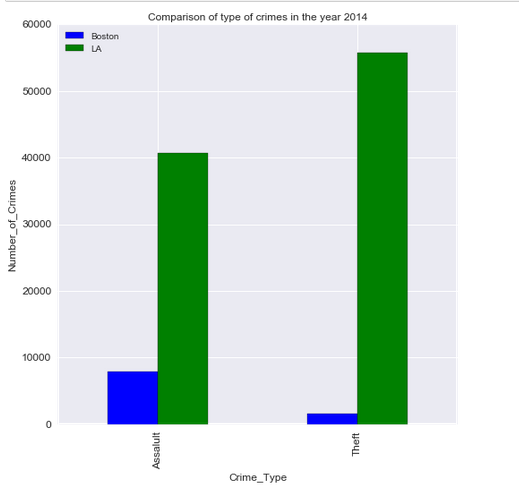
\includegraphics[width=\columnwidth]{boston-la-twotype.png}
        \caption{Comparing Assault and Thefts in Boston and Los Angeles.}
        \label{fig:tf_plot}
        \end{center}
    \end{figure}

By looking at sheer number of crimes occurring in Boston and Los Angeles, we can say Boston is relatively safer city.  We have taken 2 most common type of crimes in both the cities and plotted the above graph. It is clearly visible that LA has much more crime rate for these crimes as compared to Boston.
 

    \begin{figure}[!hbt]
        \begin{center}
        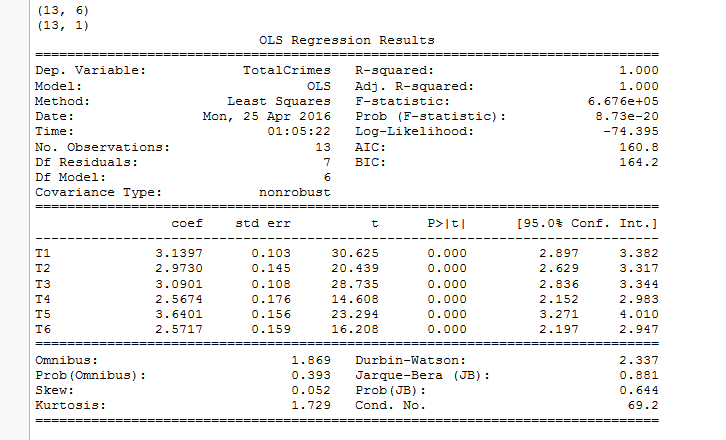
\includegraphics[width=\columnwidth]{regression-timeslot.png}
        \caption{Finding predominant timeslot using regression.}
        \label{fig:tf_plot}
        \end{center}
    \end{figure}

By looking at different timeslots, we can see that the time T5 has a higher correlation as compared to other times. This implies if an area has more number of crimes during the time period 5pm to 9pm, then that area has more chances to be unsafe.



\subsection{Results from Prediction}
    \begin{figure}[!hbt]
        \begin{center}
        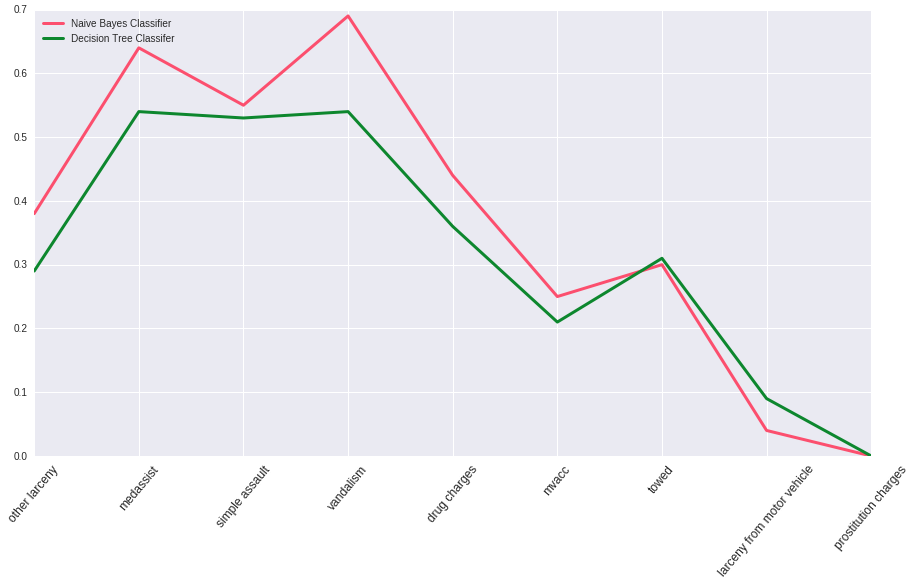
\includegraphics[width=\columnwidth]{prediction-accuracy.png}
        \caption{Output accuracy comparison for NB and DT classifiers.}
        \label{fig:tf_plot}
        \end{center}
    \end{figure}


Regarding different classifiers, the Na{\"i}ve Bayesian classifier, it achieves an
accuracy of 51\% in Boston crime prediction while it reaches 54\% for Los Angeles crime
prediction. On the other hand, decision tree classifier reports less prediction accuracy with 42 \% for Boston and 43\% for Los Angeles. Moreover, the decision tree model created a very complex tree that cannot generalize the data for both cities. However, the two classifiers have the same performance in terms of their running time. 
    \begin{figure}[!hbt]
        \begin{center}
        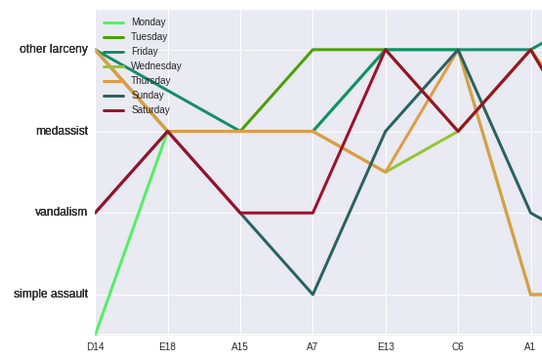
\includegraphics[width=\columnwidth]{prediction-trends.png}
        \caption{Per day trends for different areas and different crime types.}
        \label{fig:tf_plot}
        \end{center}
    \end{figure}
Above figure also shows trends for different districts within Boston. Each point stands for a prediction in certain area for certain day for certain type of crime. These seven lines passing through a single point says that type of crime is predominant in corresponding area irrespective of day of the week. E18 and C6 districts fir this description.

\section{Conclusion}
    We have now completed collecting required data, parsed it to extract required information for Boston. We have then used various analysis methods for finding patterns in criminal activities. Using different classifiers, we've also tried to use these patterns for predicting crimes. The primary are encouraging enough to pursue further techniques to get more insight on most likely next crime.
    \begin{figure}[!hbt]
        \begin{center}
        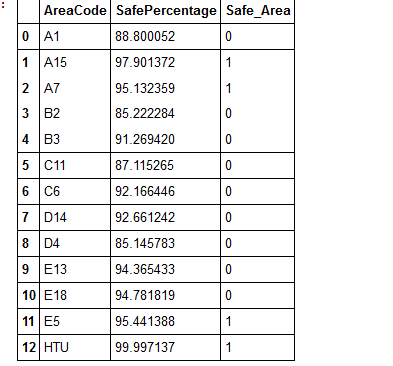
\includegraphics[width=\columnwidth]{boston-safe-area.png}
        \caption{Boston safe areas.}
        \label{fig:tf_plot}
        \end{center}
    \end{figure}
We also found which would be the safe areas in Boston. One such area is `HTU’ which is the safest of all areas in Boston. This consists of streets PARK PLAZA, BRAGDON ST, STUART ST, WASHINGTON ST and COMMONWEALTH AV.

As of now we can conclude from the Logistic Regression results, we can see that for the safe areas the only crime type that occurs in a significant number is Harassment. Also, Boston looks to be a safer city for majority of crime types in terms of frequency. But this comparison will be more accurate if we can normalize it based on population density.

Na{\"i}ve Bayes Classifier performs more accurately than Decision Tree Classifier. This accuracy can be further increased by more social data discussed in future work.

\section{Future Work}
We believe the analysis will be more accurate for multi-city data if we consider population density. Since number of crimes will vary with this factor, our analysis is not yet complete. Also, the prediction accuracy can be improved by applying external data trends. We can also see if average income, age distribution and other social aspects affect the rate and type of crimes. This can aid our prediction model while predicting crimes in specific parts of a city.
% Now we need a bibliography:
\begin{thebibliography}{5}

    %Each item starts with a \bibitem{reference} command and the details thereafter.
    \bibitem{1} % Transaction paper
    CRIME PREDICTION BASED ON CRIME TYPES AND USING SPATIAL AND  TEMPORAL CRIMINAL HOTSPOTS Tahani Almanie, Rsha Mirza and Elizabeth Lor Department of Computer Science, University of Colorado, Boulder, USA.

    \bibitem{2} 
    Crimereports.com, 2015. [Online]. Available: https://www.crimereports.com. [Accessed: 20- May-2015].
    \bibitem{3} 
    `Crime — Datasets - US City Open Data Census', Us-city.census.okfn.org, 2015. [Online]. Available: http://us-city.census.okfn.org/dataset/crime-stats. [Accessed: 20- May- 2015].
    \bibitem{4}
    Regression techniques reference. 
    \url{http://scikit-learn.org/stable/auto_examples/linear_model/plot_ols.html}
    \bibitem{5}
    GMPlot reference.
    \url{https://pypi.python.org/pypi/gmplot/1.0.5}
    
    \bibitem{6}
    GitHub code repository.
    \url{https://github.com/sahilsd/591-crime-project}

\end{thebibliography}

% Your document ends here!
\end{document}
